%%=============================================================================
%% Proof of Concept
%%=============================================================================

\chapter{\IfLanguageName{dutch}{Proof of Concept}{Proof of Concept}}%
\label{ch:proof-of-concept}

Dit deel van het onderzoek presenteert een proof of concept gericht op de beoordeling van de gekozen navigatiemethoden die gebruikt kunnen worden voor mensen met een mentale beperking. Het doel van de proof of concept is de efficiëntie, bruikbaarheid en gebruiksvriendelijkheid van deze methoden te onderzoeken aan de hand van een applicatie. De ontwikkeling van deze applicatie en hieruit gehaalde resultaten worden besproken. Als laatste zal er besproken worden welke navigatietool de meest geschikte is voor de doelgroep.

\section{Ontwikkeling van de applicatie}
\label{sec:ontwikkeling van de applicatie}
In dit onderdeel wordt de opbouw van de applicatie besproken. Hieruit zal duidelijk worden hoe de applicatie opgebouwd is. De code is niet relevant voor het verdere verloop van het onderzoek. Als eerste worden de belangrijkste onderdelen besproken. Een nieuw React Native project wordt aangemaakt aan de hand van Node.js en een terminal. Na het opzetten van dit project, moet er een Mapbox account gecreëerd worden om een publieke token te kunnen verkrijgen zodat er gebruik gemaakt kan worden van hun diverse mappen. \newline

De applicatie bestaat uit één eenvoudig scherm. Op Figuur \ref{fig:Scherm met een knop om de route op te vragen} is te zien dat er een Mapbox map ingeladen wordt en een invoerveld met een knop. Het proces wordt in gang gezet wanneer op de knop gedrukt wordt en een correct adres is ingegeven. Wanneer een foutief adres wordt ingegeven zal er een foutmelding komen en wordt het proces onderbroken. Bij Figuur \ref{fig:Scherm met knop waar route die opgevraagd is} is de route gegeneerd die op het scherm komt wanneer op de knop gedrukt wordt en een correct adres ingegeven is.

%begin{lstlisting}[caption={Code-voorbeeld van het navigatiescherm}, label=code-voorbeeld navigatiescherm, captionpos=b]
%    Mapbox.setAccessToken('MAPBOX_PUBLIC_TOKEN');
%    
%    const App = () => {
%        const [location, setLocation] = useState('');
%        const [destination, setDestination] = useState('');
%        const [route, setRoute] = useState(null);
%        const [errorMsg, setErrorMsg] = useState(null);
%        const [isLoading, setIsLoading] = useState(false);
%        
%        useEffect(() => {
%            (async () => {
%                let { status } = await Location.requestForegroundPermissionsAsync();
%                if (status !== 'granted') {
%                    setErrorMsg('Permission to access location was denied');
%                    return;
%                }
%                
%                let currentLocation;
%                if (Platform.OS === 'OS' && !__DEV__) {
%                    currentLocation = await Location.getCurrentPositionAsync({});
%                    console.log('Current location:', currentLocation);
%                } else {
%                    currentLocation = {
%                        coords: {
%                            longitude: 4.038139399999999,
%                            latitude: 50.9318886,
%                        },
%                    };
%                }
%                
%                if (!currentLocation) {
%                    setErrorMsg('Failed to obtain location');
%                    return;
%                }
%                setLocation(currentLocation);
%            })();
%        }, []);
%        
%        const getRoute = async () => {
%            setIsLoading(true);
%            const userLocation = `${location.coords.longitude},${location.coords.latitude}`;
%            console.log('User location:', userLocation);
%            
%            const YOUR_GOOGLE_API_KEY = 'GOOGLE_API_KEY';
%            
%            const startLong = location.coords.longitude;
%            const startLat = location.coords.latitude;
%            
%            try {
%                const destinationCoords = await getCoordinatesFromPlace(destination, YOUR_GOOGLE_API_KEY);
%                const endLong = destinationCoords.split(',')[1];
%                const endLat = destinationCoords.split(',')[0];
%                console.log(endLong, endLat)
%                console.log('Destination coordinates:', destinationCoords);
%                if(!destinationCoords) {
%                    throw new Error('Failed to fetch destination coordinates');
%                }
%                
%                const mapboxUrl = `https://api.mapbox.com/directions/v5/mapbox/walking/${startLong},${startLat};${endLong},${endLat}?alternatives=true&annotations=distance&continue_straight=true&geometries=geojson&overview=full&steps=false&access_token=MAPBOX_PUBLIC_TOKEN`
%                console.log('Mapbox Directions API URL:', mapboxUrl);
%                const response = await fetch(mapboxUrl);
%                const data = await response.json();
%                                
%                if (data.routes && data.routes.length > 0) {
%                    const routeCoordinates = data.routes[0].geometry.coordinates.map(coord => ({ longitude: coord[0], latitude: coord[1] }));
%                    // console.log('Route coordinates:', routeCoordinates);
%                    setRoute(routeCoordinates);
%                } else if (data.coords == 'NoRoute'){
%                    throw new Error('No route found');
%                } else {
%                    throw new Error('Failed to fetch route');
%                }
%            } catch (error) {
%                console.error(error);
%                setErrorMsg('Failed to fetch route');
%            } finally {
%                setIsLoading(false);
%            }
%        };
%        
%        const getCoordinatesFromPlace = async (place, apiKey) => {
%            const apiUrl = `https://maps.googleapis.com/maps/api/geocode/json?address=${encodeURIComponent(place)}&key=${apiKey}`;
%            
%            try {
%                const response = await fetch(apiUrl);
%                
%                console.log('Geocoding API response status:', response.status);
%                
%                if (!response.ok) {
%                    throw new Error(`Geocoding API request failed with status ${response.status}`);
%                }
%                
%                const data = await response.json();
%                                
%                if (data.status === 'OK' && data.results.length > 0) {
%                    const result = data.results.find(result => result && result.geometry && result.geometry.location);
%                    if (result) {
%                        const { lat, lng } = result.geometry.location;
%                        console.log('Geocoding result:', lat, lng);
%                        return `${lat},${lng}`;
%                    } else {
%                        throw new Error('No valid location found in the geocoding results');
%                    }
%                } else {
%                    throw new Error(`Geocoding failed: ${data.status || 'Unknown error'}`);
%                }
%            } catch (error) {
%                console.error('Error in getCoordinatesFromPlace:', error);
%                throw error;
%            }
%        };
%        
%        const renderRouteLine = () => {
%            if (!route) {
%                return null; 
%            }
%            
%            const routeCoordinates = route.map(coord => [coord.longitude, coord.latitude]);
%            // console.log("Route coordinates:", route);
%            return (
%            <Mapbox.ShapeSource id="routeSource" shape={{
%                    type: 'Feature',
%                    geometry: {
%                        type: 'LineString',
%                        coordinates: routeCoordinates,
%                    },
%            }}>
%            <Mapbox.LineLayer id="routeFill" style={{ lineColor: 'blue', lineWidth: 3 }} />
%            </Mapbox.ShapeSource>
%            );
%        };
%        
%        if (!location || !location.coords) {
%            return (
%            <View style={styles.container}>
%            <ActivityIndicator size="large" />
%            <Text>{errorMsg || 'Waiting for location...'}</Text>
%            </View>
%            );
%        }
%        
%        return (
%        <View style={styles.container}>
%        <Mapbox.MapView style={styles.map}>
%        <Mapbox.Camera
%        zoomLevel={13}
%        centerCoordinate={[location.coords.longitude, location.coords.latitude]}
%        />
%        <Mapbox.UserLocation />
%        {route && renderRouteLine()}
%        </Mapbox.MapView>
%        
%        {/* Destination Input Field */}
%        <View style={styles.inputContainer}>
%        <TextInput
%        style={styles.input}
%        placeholder="Enter destination address"
%        value={destination}
%        onChangeText={setDestination}
%        />
%        <Button title="Get Route" onPress={getRoute} disabled={isLoading} />
%        </View>
%        
%        {isLoading && (
%            <View style={styles.loading}>
%            <ActivityIndicator size="large" />
%            </View>
%            )}
%        </View>
%        );
%    };
%    
%    export default App;
%    
%    const styles = StyleSheet.create({
%        container: {
%            ...StyleSheet.absoluteFillObject,
%            justifyContent: 'flex-end',
%            alignItems: 'center',
%        },
%        map: {
%            ...StyleSheet.absoluteFillObject,
%        },
%        inputContainer: {
%            width: '100%',
%            marginBottom: 20,
%        },
%        input: {
%            width: '90%',
%            paddingHorizontal: 10,
%            borderWidth: 1,
%            borderColor: '#ccc',
%            borderRadius: 5,
%            height: 40,
%            backgroundColor: '#fff',
%            marginBottom: 10,
%        },
%        loading: {
%            position: 'absolute',
%            top: '50%',
%            left: '50%',
%            zIndex: 1,
%            transform: [{ translateX: -25 }, { translateY: -25 }],
%        },
%    });
%\end{lstlisting}


\begin{figure}[htbp]
    \centering
    \begin{minipage}[b]{0.45\textwidth}
        \centering
        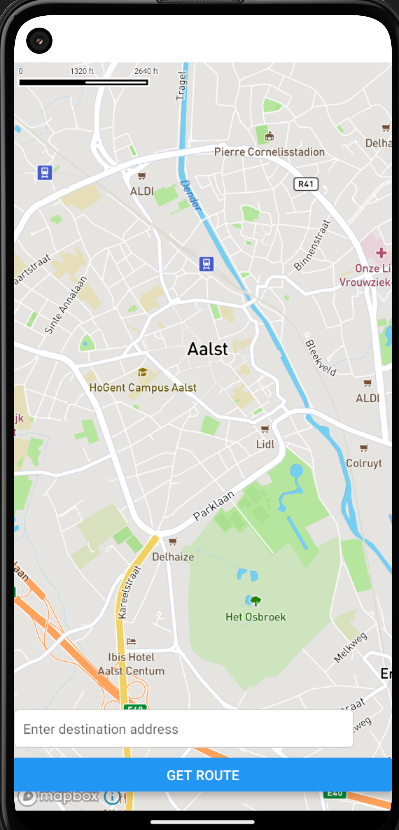
\includegraphics[width=\textwidth]{image.png}
        \caption{Scherm met een knop om de route op te vragen}
        \label{fig:Scherm met een knop om de route op te vragen}
    \end{minipage}
    \hspace{0.05\textwidth}
    \begin{minipage}[b]{0.45\textwidth}
        \centering
        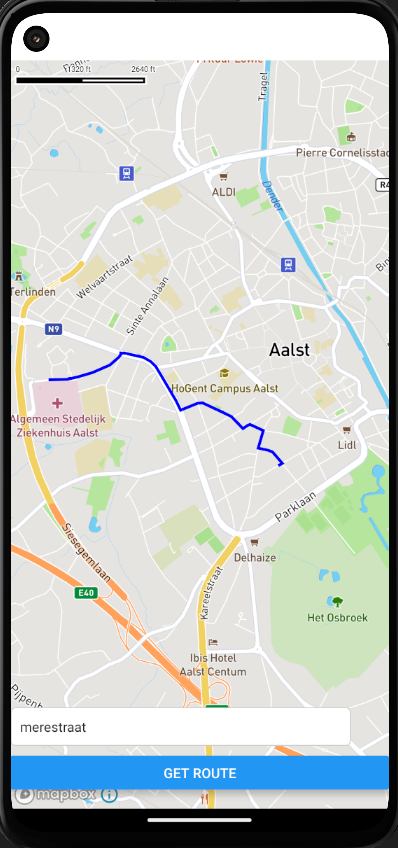
\includegraphics[width=\textwidth]{image-1.png}
        \caption{Scherm met knop waar de route die opgevraagd is}
        \label{fig:Scherm met knop waar route die opgevraagd is}
    \end{minipage}
\end{figure}

\subsection{Installatie en opstarten van de applicatie}
\label{sec:installatie en opstarten van de applicatie}

Zorg ervoor dat Node.js geïnstalleerd is op je systeem en in je \texttt{\$PATH} variabelen staat.
een Mapbox publieke token is nodig om de kaarten te kunnen gebruiken.

\begin{enumerate}
    \item Clone de repository.
    \item Voer `npm install` uit in de hoofdmap van de repository.
    \item In \texttt{App.js}, vervang 'YOUR\_MAPBOX\_PUBLIC\_KEY' door je eigen Mapbox publieke token.
    \item Bij \textbf{MapboxUrl} in \texttt{App.js}, vervang \texttt{key=YOUR\_MAPBOX\_PUBLIC\_KEY} aan het einde van de URL met je eigen Mapbox publieke token.
    \item Je hebt ook een \textbf{Google API key} \texttt{YOUR\_GOOGLE\_API\_KEY} nodig voor het maken van de route. Deze kan je verkrijgen op de Google Cloud Platform\footnote{\url{https://cloud.google.com/?hl=nl}}.
    \item Voer `npx expo start` uit om de applicatie te starten. Je kan de optie \texttt{--android} of \texttt{--ios} toevoegen om de applicatie te starten in een specifieke emulator.
    \item Selecteer een emulator of scan de QR code met de Expo app op je telefoon.
\end{enumerate}


\section{Mapbox}
\label{sec:mapbox}

\subsection*{Algemene bruikbaarheid}
\subsection*{Platform}
\subsection*{Intuïtiviteit}
\subsection*{Platformonafhankelijkheid}
\subsection*{Visuele aanwijzingen}
\subsection*{Auditieve instructies}
\subsection*{Real-time updates}
\subsection*{Toegankelijkheidsfuncties}
\subsection*{Connectiviteit}
\subsection*{Aanpasbaarheid}
\subsection*{Offline functionaliteit}
\subsection*{Veiligheidsfuncties}
\subsection*{Visual noise}
\subsection*{Speciale hardware} 
\subsection*{Het navigatieproces moet snel zijn, om tijdverlies en onzekerheid te minimaliseren}
\subsection*{De informatie die de gebruiker moet onthouden moet beperkt zijn, om het risico op fouten te verlagen}
\subsection*{Het aantal stappen in het navigatieproces moet tot een minimum beperkt blijven}
\subsection*{De navigatiemethodes moeten gebruiksvriendelijk zijn voor mensen met dyslexie. Er moet rekening gehouden worden met de lees- en onthoudmoeilijkheden die zij kunnen ervaren}
\subsection*{Het zou voordelig zijn als de navigatiemethodes kostenefficiënt zijn, zodat onnodige kosten vermeden worden, wat de dienst toegankelijker maakt voor de eindgebruiker en de aanbieder}

\section{Google Maps}
\label{sec:google maps}

\subsection*{Algemene bruikbaarheid}
\subsection*{Platform}
\subsection*{Intuïtiviteit}
\subsection*{Platformonafhankelijkheid}
\subsection*{Visuele aanwijzingen}
\subsection*{Auditieve instructies}
\subsection*{Real-time updates}
\subsection*{Toegankelijkheidsfuncties}
\subsection*{Connectiviteit}
\subsection*{Aanpasbaarheid}
\subsection*{Offline functionaliteit}
\subsection*{Veiligheidsfuncties}
\subsection*{Visual noise}
\subsection*{Speciale hardware} 
\subsection*{Het navigatieproces moet snel zijn, om tijdverlies en onzekerheid te minimaliseren}
\subsection*{De informatie die de gebruiker moet onthouden moet beperkt zijn, om het risico op fouten te verlagen}
\subsection*{Het aantal stappen in het navigatieproces moet tot een minimum beperkt blijven}
\subsection*{De navigatiemethodes moeten gebruiksvriendelijk zijn voor mensen met dyslexie. Er moet rekening gehouden worden met de lees- en onthoudmoeilijkheden die zij kunnen ervaren}
\subsection*{Het zou voordelig zijn als de navigatiemethodes kostenefficiënt zijn, zodat onnodige kosten vermeden worden, wat de dienst toegankelijker maakt voor de eindgebruiker en de aanbieder}

\section{Samenvatting}
\label{sec:samenvatting}







